\mode<article>
Normalmente es conveniente que usted presente sus resultados en un gráfico correctamente 
señalado para facilitar la lectura. En general en Matlab o python hay algún comando de 
\texttt{plot} para realizar esta tarea. Verifique también cómo anotar los ejes y escalas, como se
muestra en la \autoref{FigFrameGraficos}

\begin{figure}
  \includeslide[width=\textwidth]{FrameGraficos}
  \caption{
    \protect\label{FigFrameGraficos}
    Ejemplo de un gráfico en matlab. Se define una función partida de forma abreviada
  }


\end{figure}

\mode*

\begin{frame}<presentation>[label=FrameGraficos]
  \frametitle{Gráficos}
  \begin{columns}
    \column{0.5\textwidth}
      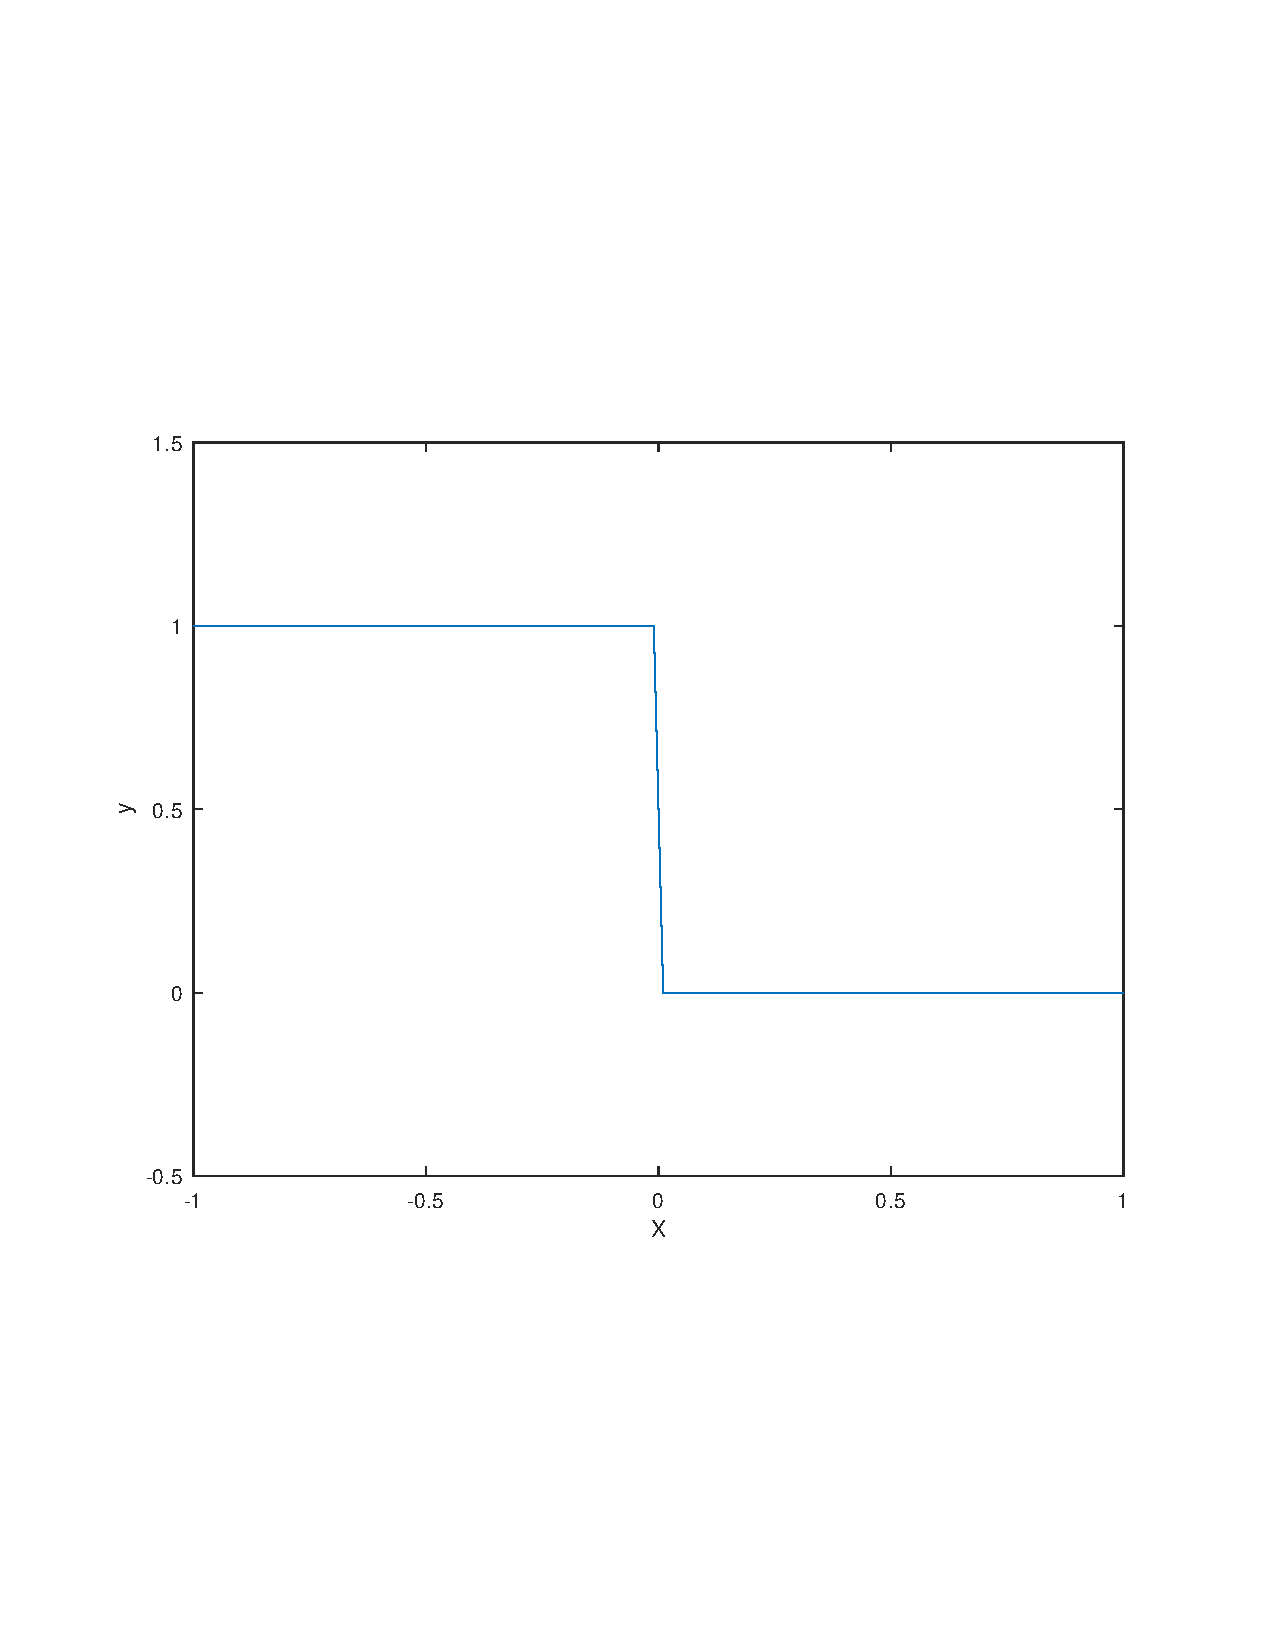
\includegraphics[width=\textwidth]{07-Graficos/partida.pdf}

    \column{0.5\textwidth}
      \begin{codeblock}
	\verbatiminput{CODEXAMPLES/plot_example.m}
      \end{codeblock}



  \end{columns}

\end{frame}

\mode<all>
